\documentclass[11pt]{article}
\usepackage{times}
\usepackage{amsmath,amsthm,amssymb,setspace,enumitem,epsfig,titlesec,verbatim,color,array,multirow,comment,graphicx}
\graphicspath{ {./images/} }
%\usepackage[super,sort&compress,comma]{natbib}
\usepackage[round, colon]{natbib}
\usepackage[bf,small]{caption}
\usepackage[export]{adjustbox}
\usepackage[top=2.5cm,left=2.6cm,right=2.6cm,bottom=3.5cm]{geometry}
\usepackage{bibunits}
\usepackage{multicol}
\usepackage{amsmath}
\usepackage{enumitem}
\smallskip

\newcommand{\christian}[1]{\textcolor{blue}{{\bf CH:} #1}} 
%\titleformat{\section}{\sffamily \fontsize{13}{20}\bfseries}{\thesection}{1em}{}
%\titleformat{\subsection}{\fontsize{11}{0}}{(\alph{subsection})}{0.4em}{\underline} 



\newtheoremstyle{plainCl1}% name
{9pt}%      Space above, empty = 'usual value'
{9pt}%      Space below
{\it}% 	   Body font
{}%         Indent amount (empty = no indent, \parindent = para indent)
{\bfseries}% Thm head font
{.}%        Punctuation after thm head
{0.2cm}% Space after thm head: \newline = linebreak
{}%         Thm head spec

\newtheoremstyle{plainCl2}% name
{9pt}%      Space above, empty = 'usual value'
{9pt}%      Space below
{\it}% 	   Body font
{}%         Indent amount (empty = no indent, \parindent = para indent)
{\bfseries}% Thm head font
{$'$.}%        Punctuation after thm head
{0.2cm}% Space after thm head: \newline = linebreak
{}%         Thm head spec


\theoremstyle{plainCl1}
\newtheorem{Claim}{Claim}
\newtheorem{Thm}{Theorem}
\newtheorem{Prop}{Proposition}
\newtheorem{Lem}{Lemma}
\newtheorem{Cor}{Corrolary}






\title{Consistency and Trust}
\date{\today}
\author{CR MH CH}


\begin{document}
\maketitle
\onehalfspacing

\section{Predictions}

\paragraph{Actor}

\begin{enumerate}
    \item The more consistent in his cooperative actions the actor is, the more consistent he will be in future action.
    \item After a betrayal/cheating, the actor has no incentives to be consistent in his cooperative behaviour again and will not be. 
\end{enumerate}

\paragraph{Observer}

\begin{enumerate}
    \item As the actor keeps behaving consistently, the observer's trust increases.
    \item The first defection reduces how moral/trustworthy they find the person much more so than the second defection.
    \item In the rare case where the actor tries to rebuild trust/consistency after a betrayal/cheating, the observer will never regain full trust again.
    \item Conditional trust: how does one cooperative action increase trust vs how does one betrayal/cheating action decrease trust (difference of a difference)
\end{enumerate}

\section{Current experimental design}

\noindent
At this stage, we are only interested in testing the predictions of the actor/sender. Specifically we want to check that:
\begin{enumerate}
    \item The more the sender cooperated in previous rounds, the more likely to cooperate now.
    \item After just one defection, the sender "never" cooperate again.
    \item monotonicity - when are costs higher, the sender cooperates less. 
\end{enumerate}

\subsection{Key elements}

\paragraph{Dictator Game}
We use a multi round DG reframed as a take rather give scenario to highlight the non desirability of the action. 
On every round, by default the two players have a half-spilt of the total pot. 
The dictator can choose to either leave it like that or steal the money of the recipient. It is important that a high enough amount of participant do steal in this design to be able to detect an effect.

\paragraph{k rounds}
For now 2 suffice to test consistency. 
we manipulate the number of rounds, but we could manipulate other things such as plausible deniability (to test intention) 
and observability (by a third party or someone who will interact with the sender later).\

\paragraph{stochastic cost levels}
2 suffice: low vs high. \\
The value of the cost must change across rounds in order to test consistency. 
At the moment the cost and benefit ratios are the same for both the high and low cost. \\
It's possible to have these costs be randomly assigned, but we would end up with combinations of high and low cost that do not serve any predictions. 
To avoid that, we can fix the combinations of costs that we need into treatments. This way we do not lose money and data points. 
However, the issue now is that which cost one encounters in a given round is not random. Only treatment assignment is. 
This means that we must be careful about what we tell our participants about the distribution of these costs. 
There is a tradeoff between what is convenient/cheaper and the level of deception we are willing to tolerate.\\
We also need to make sure that when the costs are higher, there is less cooperation (monotonicity).
Players must be more likely to cooperate when the costs are lower than when they are higher. 

\paragraph{cooperative choices with different partners}
We have a perfect random matching design. 

\paragraph{assume "zero-tolerance" }
Something we need to check and be able to rule out is that some people might just cooperate more. 
We must be able to manipulate the degree of "zero-tolerance" to show that is doesn't merely reflect individual difference and rule that out as a possible confound. \\
we must show that there is no licensing as well. 

\subsection{Testing}

In practice it looks like that:

\noindent
\textbf{Sender cooperate more when facing a high low cost.} \\
We compare cooperation rates in the first round between treatments that faced a low or a high cost first. \\

\noindent
\textbf{Sender more likely to cooperate in round 2 when round one had a low cost AND they cooperated.} \\
Two different comparisons:
\begin{enumerate}
    \item \textbf{low-low vs high-low} (compare round 2 cooperation across the two treatments)\\ 
    		We expect to find a difference in cooperation rates on round 2 between these two treatments based on what they faced in the first round and if they cooperated or not (coop if low 			and defect if high). We can also show that sender lose motivation after defecting.
    \item \textbf{low-high vs high-any} (compare the cooperation rate in the two high cost rounds across treatments)
    		Moreover, fully mediated by whether defected in prior rounds. 
		By having the same definite cost on an early round vs a later round the sender can build social capital.
\end{enumerate}

\section{Design considerations for later}

\subsection{Potential games}
In order to test the predictions above, we need a two-player game that induces a high amount of cheating/defection. There are three candidates:

\paragraph{Cheating task}

If the dictator game does not induce enough cheating/defecting, we could use a task specifically designed to test cheating behaviour. 
There exists are few different ones, we would have to discuss which ones fit best. See Mazar and Gneezy papers for examples.
\begin{itemize}
    \item either a task in pairs where one has the opportunity to directly lie to the other
    \item or one does a task where he can cheat, and the other player may or may not be able to observe that
\end{itemize}
Advantage: we add principle (Lying/cheating is universally considered bad). 

\paragraph{Trust Game}

Finally a trust game might be game we ultimately use. Just as with the dictator game we have different costs to test consistency. 
The advantage of the Trust game is that the recipient is now an active player and that trust can be measured directly (by the money sent back). 

\subsection{Other considerations}

\paragraph{Observer}
\begin{itemize}
    \item The observer may or may not know the level of temptation of the actor (= cost on each round)
    \item The observer can be a third party who learns the history of play or the interaction partner who would have to know previous actions. 
    \item We need to measure the observer's level of trust
    	\begin{itemize}
	\item Partner choice (choose who to they want to be paired with to play another DG)
	\item Add a second stage and make it a trust game
    	\item Character judgment (asking directly to rate trustworthiness or morality)
	\item Ask observer what how they expect the Actor to act
    	\end{itemize}
    \item We need to manipulate the history of play for the actor. 
    	\begin{itemize}
	\item Strategy method (ask what they expect the actor will do for every possible scenario)
	\item Hope enough subjects behave in all possible ways
    	\item Use deception
    	\end{itemize}
\end{itemize}


\section{Model}

\subsection{Description of the signaling game}


In the following we describe a simple signaling game. The game involves two players, a sender and a receiver. It consists of several rounds in which senders can decide whether or not to send a costly signal. The exact cost in a given round is determined randomly and may depend on the type of the sender. We use this model to explore under which conditions we observe equilibria that show the characteristics of principled behavior, discontinuity and complementarity. In addition, the same model will also allow us to characterize other equilibria of interest (such as equilibria with moral licensing).
The game proceeds as follows. 

\begin{description}
\item[Stage 0: Move of nature.] We assume that senders can be of two different types, they are either of the superior ($S$) or of the inferior ($I$) type. The type of the sender is randomly determined before the game starts. Let $p_S$ be the probability that a given sender is superior. Senders learn their own type, but receivers do not know the type of sender they interact with. 
\item[Stage 1--n: Signaling rounds.] After the sender's type is determined, the sender faces $n$ opportunities in which she can signal her type to the receiver. Each of these $n$ rounds proceeds as follows:\\
First nature randomly determines the cost of the signal; this cost can be either low or high, $c\!\in\!\{c_l,c_h\}$ with $c_h\!>\!c_l\!>\!0$. The probability of having a high cost is independent of the round number and of previous realized costs. However, it depends on the type of the sender; superior senders experience a high cost with probability $q_{S,h}$, whereas this probability is $q_{I,h}$ for inferior types. We use $q_{S,l}=1-q_{S,h}$ and $q_{I,l}=1-q_{I,h}$ for the probability that the respective cost is low. 
Moreover, we use $\bar{c}_\theta:=q_{\theta,l} c_l + q_{\theta,h} c_h$ to denote the expected cost that a sender of type $\theta$ experiences in any given round. 
In the following we assume $q_{S,h}\!\le\!q_{I,h}$. 
That is, superior types are less likely to experience a high cost. The sender (but not the receiver) learns the exact cost. Then the sender decides whether or not to pay the cost in order to send the signal. 
\item[Stage $n+1$: Receiver's decision.] After the sender has made her decisions, the receiver learns in how many of the $n$ rounds the sender paid the signaling cost. The receiver then decides whether or not to accept the sender. If the receiver rejects the sender, the payoffs in that final stage are zero for both players. If he accepts the sender, the payoffs depend on the sender's type; the sender's payoff is $a_\theta$ and the receiver's payoff is $b_\theta$ with $\theta\in\{S,I\}$. 
Receivers get a positive payoff from accepting superior senders, but a negative payoff from accepting inferior senders, $b_S > 0 > b_I$. 
\end{description}

\noindent
In the following, we assume the senders' strategies take the form $\mathbf{\sigma}_\theta = \sigma_\theta(i,k,c)$. 
Here, the input $i\in\{1,\ldots,n\}$ is the given round for which a decision is to be made; $k\in\{0,\ldots,i-1\}$ is the number of times a signal has been sent in the past, and $c\in\{c_l, c_h\}$ is the current cost. The output takes the form $\sigma_\theta(i,k,c) \in \{0,1\}$ where 0 refers to not sending the signal for the given input. 
The receiver's strategy takes the form $\mathbf{\rho} = \rho(k)$, where $k\in\{0,\ldots,n\}$ refers to the number of times the sender has sent the signal. Here, the output again takes values  $\rho(k)\in\{0,1\}$, where $0$ means to reject the sender. 


% Possible place to further motivate this model and discuss other variants that would give comparable results. 

\subsection{The case of two rounds}

In the following, we first study the case in which there are two rounds only, $n\!=\!2$. We are interested in the following strategy profile
\begin{equation}
\sigma_S(i,k,c) = \left\{
\begin{array}{ll}
1	&\text{if}~k=i-1\\
0	&\text{otherwise}
\end{array}
\right.
\end{equation}
\begin{equation}
\sigma_I(i,k,c)= \left\{
\begin{array}{ll}
1	&\text{if}~(i\!=\!1 ~\text{and}~ c\!=\!c_l)~\text{or}~(i\!=\!2~\text{and}~k\!=\!1)\\
0	&\text{otherwise}
\end{array}
\right.
\end{equation}
\begin{equation}
\rho(k) = \left\{
\begin{array}{ll}
1	&\text{if}~k=n\\
0	&\text{otherwise}
\end{array}
\right.
\end{equation}
We refer to the above strategy profile as the `zero tolerance profile'. 

\begin{Claim}
The zero tolerance profile is a perfect Bayesian Nash equilibrium if and only if the following conditions hold:
\begin{equation}
\begin{array}{c}
\displaystyle \frac{b_S}{-b_I} \ge \frac{q_{I,l}(1\!-\!p_S)}{p_S}\\[0.4cm]
\displaystyle a_S \ge c_h +  \bar{c}_S\\[0.4cm]
\displaystyle  c_h +  \bar{c}_I \ge a_I \ge c_l + \bar{c}_I. 
\end{array}
\end{equation}
\end{Claim}

\noindent
All proof are provided in the {\bf Appendix.} Here, we give the interpretation of these conditions. The first condition states that the receiver finds it worthwhile to accept if they observe their co-player sent the signal in both rounds. The second condition states that superior senders are willing to pay the high cost even if it occurs in the first round. The last condition states that the inferior sender would be willing to pay the low cost but not the high cost.\\

\noindent
We are also interested in the following profile:
\begin{equation}
\sigma_S(i,k,c) = \left\{
\begin{array}{ll}
1	&\text{if}~(i\!=\!1 ~\text{and}~ c\!=\!c_l)~\text{or}~(i\!=\!2~\text{and}~k\!=\!0)\\
0	&\text{otherwise}
\end{array}
\right.
\end{equation}
\begin{equation}
\sigma_I(i,k,c)= \left\{
\begin{array}{ll}
1	&\text{otherwise}\\
0	&\text{if}~ c\!=\!c_h~\text{or}~(i\!=\!2~\text{and}~k\!=\!1)
\end{array}
\right.
\end{equation}
\begin{equation}
\rho(k) = \left\{
\begin{array}{ll}
1	&\text{if}~k \ge n-1\\
0	&\text{otherwise}
\end{array}
\right.
\end{equation}
We refer to the above strategy profile as the `licensing profile'. 

\begin{Claim}
The licensing profile is a perfect Bayesian Nash equilibrium if and only if the following conditions hold:
\begin{equation}
\begin{array}{c}
\displaystyle \frac{b_S}{-b_I} \ge \frac{q_{I,l}(1\!-\!p_S)}{p_S}\\[0.4cm]
\displaystyle a_I \le q_{I,l}(a_I-c_l)+c_h\\[0.4cm]
\displaystyle  c_h \ge \bar{c}_S \ge c_l. 
\end{array}
\end{equation}
\end{Claim}

\noindent
All proof are provided in the {\bf Appendix.} Here, we give the interpretation of these conditions. \\

\noindent{Further notes on how to continue:}
\begin{enumerate}
\item Write the proof of Claim 1 (CR)
\item Talk about complementarity and discontinuity in the context of the model.
\item Create analogous claim for licensing equilibrium (CR)
\item Ideally, characterize all equilibria, given natural assumptions. 
\item Describe some characteristics of equilibria (e.g., when does being an equilibrium plus Eq. [3] imply Eqs. [1]-[2])
\end{enumerate}



\subsubsection{The game}

\begin{enumerate}[label={(\alph*)}]
\item Model
	\begin{enumerate}[label={(\arabic*)}]
    	\item Players: Two players: Sender \& Receiver\\
		Sender can be of two types: Superior $S$ \& Inferior $I$ and $p^S + p^I = 1 $
    	\item Actions: 2 rounds in which sender can cooperate (c) or defect (d)\\
		Afterwards, Receiver accepts or rejects.
   	\item Order of moves: 
		\begin{table}[h]
		\centering
		\begin{tabular}{llll}
		            & (0)  & Nature determines types of Senders   &   \\
		Round 1     & (1a) & Nature determines costs              &   \\
		            & (1b) & Sender decides whether to cooperate~ &   \\
		Round 2     & (2a) & Nature determines costs              &   \\
		            & (2b) & Sender decides whether to cooperate  &   \\
		Final stage & (3)  & Receiver decides whether to accept   &  
		\end{tabular}
		\end{table}
	\item Information that the players have:
		\begin{multicols}{2}
		Sender
		\begin{itemize}
		\item Own type
		\item Current cost
		\item Previous action
		\end{itemize}
		\columnbreak
		Receiver
		\begin{itemize}
		\item Actions of the Sender
		\end{itemize}
		\end{multicols}
		\item Payoffs:
			\begin{itemize}
			\item Costs
			\item Payoffs if rejected \quad $(0,0)$
			\item Payoff if accepted \quad  $\underset{(a^I, -b^I) }{(a^S, b^S)}$ \quad $\underset{b^I > 0}{b^S > 0}$
			\end{itemize}
	\end{enumerate}
\item Assumptions
	\begin{enumerate}[label={(\arabic*)}]
	\item Receivers only want to pair with superior Senders \quad $b^S > 0 > -b^I$
	\item Senders are generally willing to signal \quad $2c_l > a^t$
	\item Some signalling is required \quad $p^S b^S - p^I b^I <0$
	\item Inferior senders do not signal at all costs \quad $2c_h < a^I$
	\end{enumerate}
	
\item Specify players' strategies
	\begin{equation}\label{strategies2}
	\begin{array}{l}	
	\sigma^S = (\sigma^{S1}_h, \sigma^{S1}_l, \sigma^{S2}_{hc}, \sigma^{S2}_{hd}, \sigma^{S2}_{lc}, \sigma^{S2}_{ld})\\
	\sigma^I = (\sigma^{I1}_h, \sigma^{I1}_l, \sigma^{I2}_{hc}, \sigma^{I2}_{hd}, \sigma^{I2}_{lc}, \sigma^{I2}_{ld})\\
	\rho = (\rho_{cc}, \rho_{cd}, \rho_{dc}, \rho_{dd})
	\end{array}
	\end{equation}
	where $S,I$ is the Sender's type, $1,2$ the round number, $h,l$ the cost on that round, and $c,d$ the action on the previous round.
\item Properties:
	\begin{enumerate}[label={(\arabic*)}]
	    \item Threshold \quad 
	    \item Betweenness \quad
	    \item Complementarity \quad $\sigma^{\theta,n+1}_{(c,..,c)} > \sigma^{\theta,n}_{(c,..,c)} \forall n$
	    \item Discontinuity \quad $\sigma^{\theta,n}_{h} = \underbar{c}$ \quad $\forall h: D \in h$
	    \item Existence of committed type \quad $\sigma^{S,n} = \bar{c}$
	    \item licensing (inverse of complementarity) \quad $\sigma^{\theta,n}_{h} < \sigma^{\theta,n}_{(d,...,d)}$ \quad $h$ such that $c \in h$
	    \item Anti-complementarity \quad $\exists n$ \quad $\sigma^{\theta,n+1}_{(c,..,c)} < \sigma^{\theta,n}_{(c,..,c)}$
	    \item Monotonicity in types \quad $\sigma^{S,n}_{h} > \sigma^{I,n}_{h}$
	\end{enumerate}
\end{enumerate}


\subsection{Signalling Game with 3 rounds}
\subsubsection{The game}

Equivalent to the 2 rounds version but the Sender gets an additional thrid round to send the signal or not. Players, Actions, Informations and Payoffs stay the same. 

\begin{enumerate}[label={(\alph*)}]
\item New strategies
	\begin{equation}\label{strategies3}
	\begin{array}{l}	
	\sigma^S = (\sigma^{S1}_h, \sigma^{S1}_l, \sigma^{S2}_{hc}, \sigma^{S2}_{hd}, \sigma^{S2}_{lc}, \sigma^{S2}_{ld}, 
	\sigma^{S3}_{hcc}, \sigma^{S3}_{hcd}, \sigma^{S3}_{hdc}, \sigma^{S3}_{hdd}, \sigma^{S3}_{lcc}, \sigma^{S3}_{lcd}, , \sigma^{S3}_{ldc}, \sigma^{S3}_{ldd})\\
	\sigma^I = (\sigma^{I1}_h, \sigma^{I1}_l, \sigma^{I2}_{hc}, \sigma^{I2}_{hd}, \sigma^{I2}_{lc}, \sigma^{I2}_{ld}, 
	\sigma^{I3}_{hcc}, \sigma^{I3}_{hcd}, \sigma^{I3}_{hdc}, \sigma^{I3}_{hdd}, \sigma^{I3}_{lcc}, \sigma^{I3}_{lcd}, , \sigma^{I3}_{ldc}, \sigma^{I3}_{ldd})\\
	\rho = (\rho_{ccc}, \rho_{ccd}, \rho_{cdc}, \rho_{cdd}, \rho_{dcc}, \rho_{dcd}, \rho_{ddc}, \rho_{ddd})
	\end{array}
	\end{equation}
	where $S,I$ is the Sender's type, $1,2,3$ the round number, $h,l$ the cost on that round, and $c,d$ the action on the two previous rounds.
\end{enumerate}

\subsubsection{Equilibrium analysis}
\paragraph{1st equilibrium of interest}
The superior type cooperates on the first round regardless of costs, and then cooperates in subsequent rounds as long as he cooperated in all previous rounds. If he defected once, he does not cooperate. The Inferior type cooperates on the first round only when he sees a low cost. He cooperates on subsequent round in the same fashion as the superior type. The Receiver accept only and only if there are no defections at all.\\
	\begin{equation}\label{strategies}
	\begin{array}{l}	
	\sigma^S = (1, 1, 1, 0, 1, 0, 1, 0, 0, 0)\\
	\sigma^I = (0, 1, 1, 0, 1, 0, 1, 0, 0, 0)\\
	\rho = (1, 0, 0, 0, 0, 0, 0, 0)
	\end{array}
	\end{equation}
We get:\\	
Receiver:
\begin{itemize} [noitemsep]
	\item Receiver after $ccc \quad \rightarrow \quad accept \quad \rightarrow \quad \frac{b^S}{b^I}\geq \frac{q^I_l (1-p_S)}{P_S}$\\
	\item Receiver after $ccd, cdc, dcc, cdd, dcd, ddc, ddd \quad \rightarrow \quad reject \quad \rightarrow \quad -b^I \geq 0$\\
\end{itemize}
Superior \& Inferior Sender on Round 3:
\begin{itemize} [noitemsep]
	\item Sender after $cc$ in $r_{1,2}$ and $C_h$ now $\quad \rightarrow \quad cooperate \quad \rightarrow \quad C_h \leq a^S$\\
	\item Sender after $cc$ in $r_{1,2}$ and $C_l$ now $\quad \rightarrow \quad cooperate \quad \rightarrow \quad C_l \leq a^S$\\
	\item Sender after $cd, dc, dd$ in $r_{1,2}$ and $C_h$ now $\quad \rightarrow \quad defect \quad \rightarrow \quad 0 \geq C_h$\\
	\item Sender after $cd, dc, dd$ in $r_{1,2}$ and $C_l$ now $\quad \rightarrow \quad defect \quad \rightarrow \quad 0 \geq C_l$\\
\end{itemize}
Superior \& Inferior Sender on Round 2:
\begin{itemize} [noitemsep]
	\item Sender after $d$ in $r_1$ and $C_h$ now $\quad \rightarrow \quad defect \quad \rightarrow \quad C_h \leq 0$\\
	\item Sender after $d$ in $r_1$ and $C_l$ now $\quad \rightarrow \quad defect \quad \rightarrow \quad C_l \leq 0$\\
	\item Sender after $c$ in $r_1$ and $C_h$ now $\quad \rightarrow \quad cooperate \quad \rightarrow \quad a^S \geq C_h q^S_h + C_l q^S_l + C_h$\\
	\item Sender after $c$ in $r_1$ and $C_l$ now $\quad \rightarrow \quad cooperate \quad \rightarrow \quad a^S \geq C_h q^S_h + C_l q^S_l + C_l$\\
\end{itemize}
Superior Sender on Round 1:
\begin{itemize} [noitemsep]
	\item Sender after $C_h$ now $\quad \rightarrow \quad cooperate \quad \rightarrow \quad a^S \geq C_h q^S_h + C_l q^S_l  + C_h q^S_h + C_l q^S_l + C_h$\\
	\item Sender after $C_l$ now $\quad \rightarrow \quad cooperate \quad \rightarrow \quad a^S \geq C_h q^S_h + C_l q^S_l  + C_h q^S_h + C_l q^S_l + C_l$\\
\end{itemize}
Inferior Sender on Round 1:
\begin{itemize} [noitemsep]
	\item Sender after $C_h$ now $\quad \rightarrow \quad defect \quad \rightarrow \quad a^I \leq C_h q^I_h + C_l q^I_l  + C_h q^I_h + C_l q^I_l + C_h$\\
	\item Sender after $C_l$ now $\quad \rightarrow \quad cooperate \quad \rightarrow \quad a^I \geq C_h q^I_h + C_l q^I_l  + C_h q^I_h + C_l q^I_l + C_l$\\
\end{itemize}


\paragraph{2nd equilibrium of interest} 
Same as above for the Superior type and the Receiver. But now the inferior type may cooperate in the second round even after a defection in the first round.\\
	\begin{equation}\label{strategies}
	\begin{array}{l}	
	\sigma^S = (1, 1, 1, 0, 1, 0, 1, 0, 0, 0)\\
	\sigma^I = (0, 1, 1, 0, 1, 0, 1, 0, 0, 0)\\
	\rho = (1, 0, 0, 0, 0, 0, 0, 0)
	\end{array}
	\end{equation}


\section{Appendices}

\subsection{Proofs}

\paragraph{Claim 1}zero-tolerance equilibrium:\\
Receiver:
\begin{itemize} [noitemsep]
	\item Receiver after $cc \quad \rightarrow \quad accept \quad \rightarrow \quad \frac{b^S}{b^I}\geq \frac{q^I_l (1-p_S)}{P_S}$\\
	\item Receiver after $cd, dc, dd \quad \rightarrow \quad reject \quad \rightarrow \quad -b^I \geq 0$\\
\end{itemize}
Superior \& Inferior Sender on Round 2:
\begin{itemize} [noitemsep]
	\item Sender after $d$ in $r_1$ and $C_h$ now $\quad \rightarrow \quad defect \quad \rightarrow \quad C_h \leq 0$\\
	\item Sender after $d$ in $r_1$ and $C_l$ now $\quad \rightarrow \quad defect \quad \rightarrow \quad C_l \leq 0$\\
	\item Sender  after $c$ in $r_1$ and $C_h$ now $\quad \rightarrow \quad cooperate \quad \rightarrow \quad a^S \geq C_h$\\
	\item Sender  after $c$ in $r_1$ and $C_l$ now $\quad \rightarrow \quad cooperate \quad \rightarrow \quad a^S \geq C_l$\\
\end{itemize}
Superior Sender on Round 1:
\begin{itemize} [noitemsep]
	\item Sender after $C_h$ now $\quad \rightarrow \quad cooperate \quad \rightarrow \quad a^S \geq C_h q^S_h + C_l q^S_l + C_h$\\
	\item Sender after $C_l$ now $\quad \rightarrow \quad cooperate \quad \rightarrow \quad a^S \geq C_h q^S_h + C_l q^S_l + C_l$\\
\end{itemize}
Inferior Sender on Round 1:
\begin{itemize} [noitemsep]
	\item Sender after $C_h$ now $\quad \rightarrow \quad defect \quad \rightarrow \quad a^I \leq C_h q^I_h + C_l q^I_l + C_h$\\
	\item Sender after $C_l$ now $\quad \rightarrow \quad cooperate \quad \rightarrow \quad a^I \geq C_h q^I_h + C_l q^I_l + C_l$\\
\end{itemize}

\paragraph{Claim 2} licensing equilibrium:\\
Receiver:
\begin{itemize} [noitemsep]
	\item Receiver after $cc \quad \rightarrow \quad$ Out of equilibrium!\\
	\item Receiver after $cd, dc \quad \rightarrow \quad accept \quad \rightarrow \quad ???$\\
	\item Receiver after $dd \quad \rightarrow \quad reject \quad \rightarrow \quad -b^I \geq 0$\\
\end{itemize}
Superior Sender on Round 2:
\begin{itemize} [noitemsep]
	\item Sender after $c$ in $r_1$ and $C_h$ now $\quad \rightarrow \quad defect \quad \rightarrow \quad C_h \leq 0$\\
	\item Sender after $c$ in $r_1$ and $C_l$ now $\quad \rightarrow \quad defect \quad \rightarrow \quad C_l \leq 0$\\
	\item Sender  after $d$ in $r_1$ and $C_h$ now $\quad \rightarrow \quad cooperate \quad \rightarrow \quad a^S \leq C_h$\\
	\item Sender  after $d$ in $r_1$ and $C_l$ now $\quad \rightarrow \quad cooperate \quad \rightarrow \quad a^S \leq C_l$\\
\end{itemize}
Inferior Sender on Round 2:
\begin{itemize} [noitemsep]
	\item Sender  after $d$ in $r_1$ and $C_l$ now $\quad \rightarrow \quad defect \quad \rightarrow \quad a^I \geq C_h$\\
\end{itemize}
Superior Sender on Round 1:
\begin{itemize} [noitemsep]
	\item Sender after $C_h$ now $\quad \rightarrow \quad defect \quad \rightarrow \quad  C_h \geq -C_h q^S_h - C_l q^S_l$\\
	\item Sender after $C_l$ now $\quad \rightarrow \quad cooperate \quad \rightarrow \quad  C_l \leq -C_h q^S_h - C_l q^S_l$\\
\end{itemize}
Inferior Sender on Round 1:
\begin{itemize} [noitemsep]
	\item Sender after $C_h$ now $\quad \rightarrow \quad defect \quad \rightarrow \quad a^I \geq q^I_l (-C_l + a^I) + C_h$\\
	\item Sender after $C_l$ now $\quad \rightarrow \quad cooperate \quad \rightarrow \quad C_l \leq -C_h q^I_h - C_l q^I_l$\\
\end{itemize}






\section{oTree Screenshots}

\begin{figure}[h]
\centering
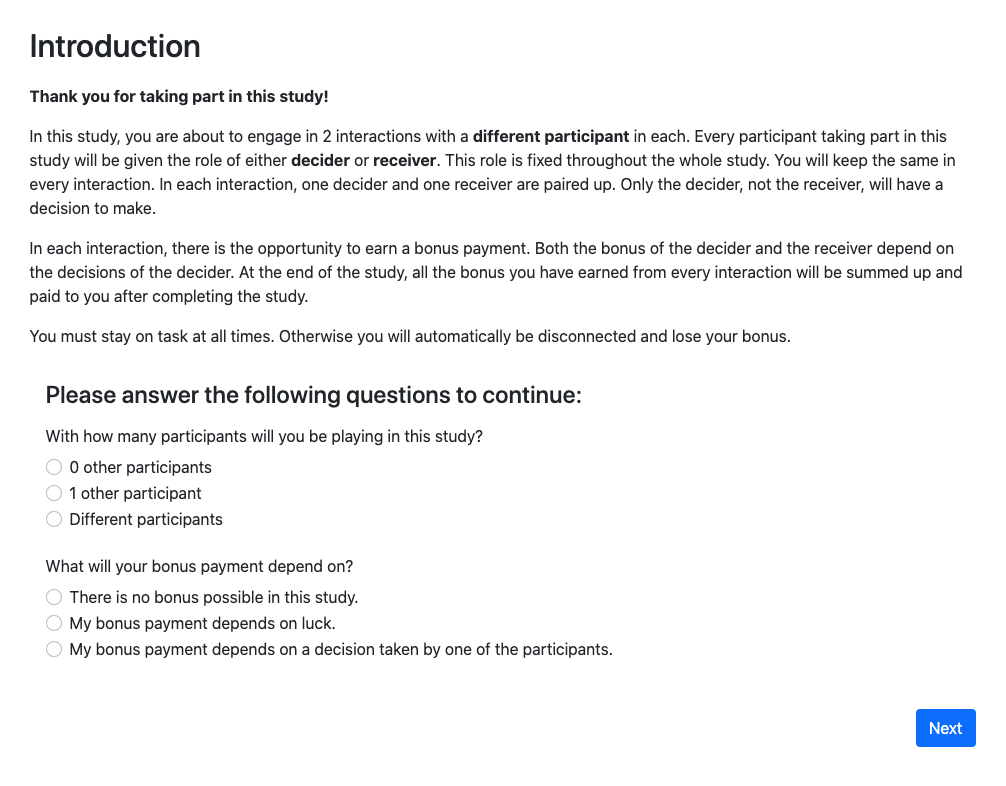
\includegraphics[scale=0.5]{welcome}
\end{figure}

\begin{figure}[h]
\centering
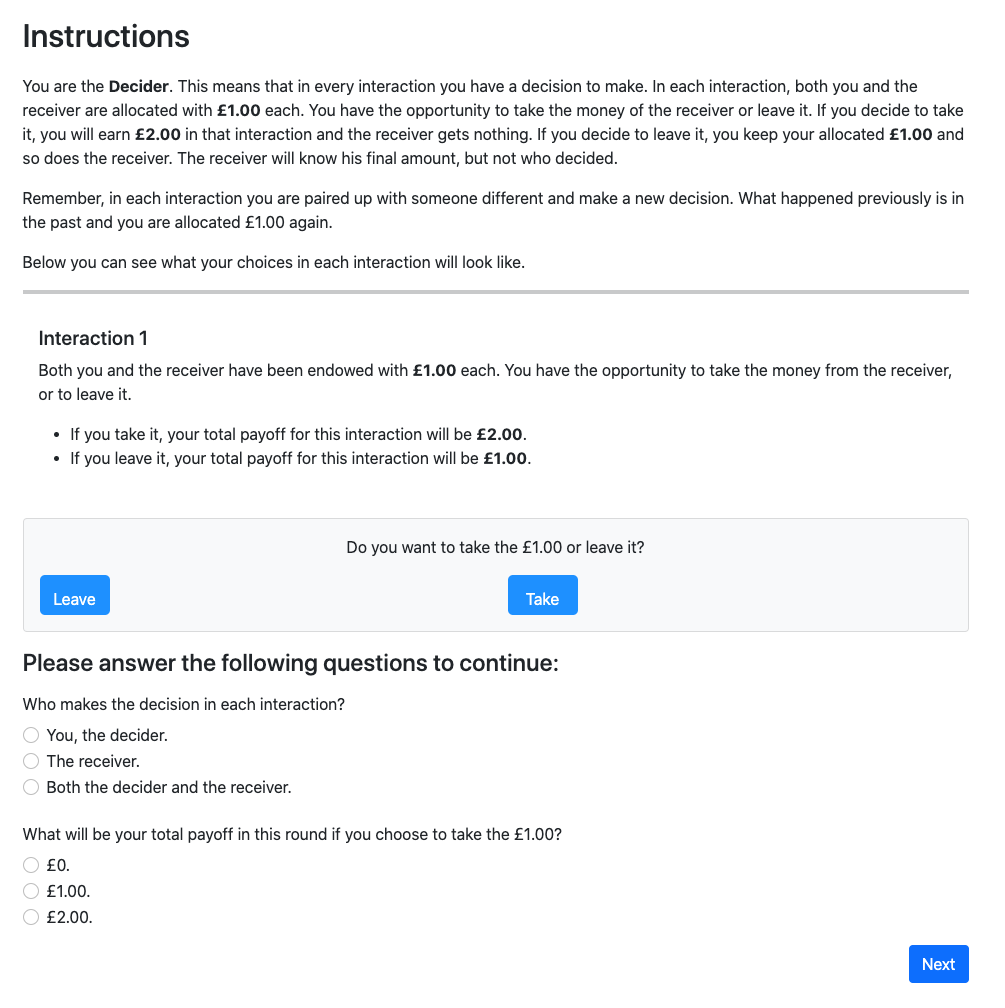
\includegraphics[scale=0.5]{instructions}
\end{figure}

\begin{figure}[h]
\centering

\includegraphics[scale=0.5]{decision_high}
\end{figure}

\begin{figure}[h]
\centering

\includegraphics[scale=0.5]{decision_low}
\end{figure}

\begin{figure}[h]
\centering

\includegraphics[scale=0.5]{results_high_take}
\end{figure}

\begin{figure}[h]
\centering

\includegraphics[scale=0.5]{results_high_leave}
\end{figure}

\begin{figure}[h]
\centering
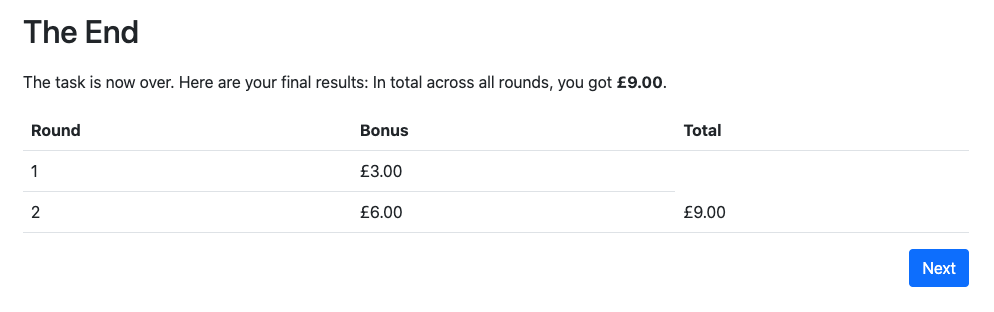
\includegraphics[scale=0.5]{end}
\end{figure}

\begin{figure}[h]
\centering
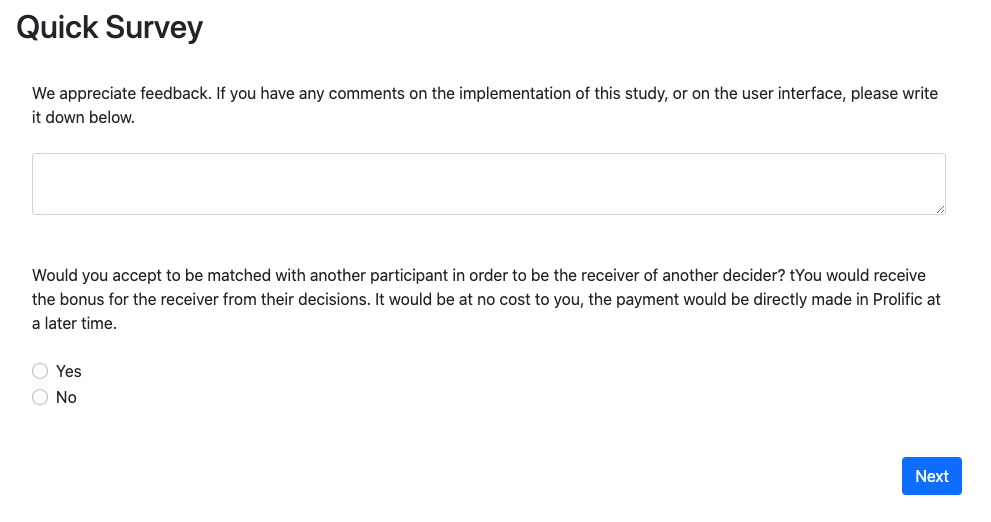
\includegraphics[scale=0.5]{commentbox}
\end{figure}

\begin{figure}[h]
\centering
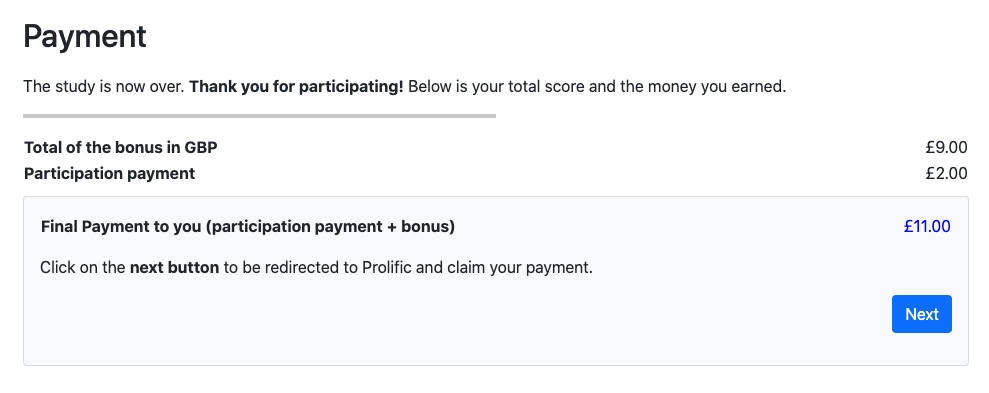
\includegraphics[scale=0.5]{payment}
\end{figure}




\end{document}
















